In the forthcoming deployment of WebRTC systems, we speculate that high
quality\footnote{normally, corresponds to increase in required bandwidth}
video conferencing will see wide adoption. Normally, to assure stability of the
network (and avoid congestion collapse), these real-time communication systems
need to implement some kind of congestion control for their RTP-based media
traffic.

RTP transmits the media data over IP using a variety of transport layer
protocols such as UDP, TCP, and Datagram Congestion Control Protocol (DCCP).
Consequently, congestion control for RTP-based media flows is implemented
either in the application or the media flows are transmitted over
congestion-controlled transport (TCP or DCCP). While using a congestion
controlled transport may be safe for the network, it is suboptimal for the
media quality unless the congestion-controlled transport is designed to carry
media flows. Unfortunately, TCP is only suitable for interactive multimedia
for paths with very low RTT ($<100$ms)~\cite{Brosh:tcp-real-time}, and DCCP
packets has problems with NAT traversal~\cite{schier:DCCP} unless DCCP is
encapsulated in UDP~\cite{RFC6773}.

This motivates the need for a UDP congestion control, where the congestion
control is implemented in-between the application and the underlying
transport. Thereby the congestion control algorithm takes into account both
the application's and the transport's requirements/constraints and make the
appropriate trade-off. In this thesis, we consider congestion control for
unicast RTP traffic running over best-effort IP network.

% CC should not cause queuing delay. Or define low-latency operation of
% multimedia cc.

Endpoints rely on RTCP feedback from the receiver to implement congestion
control. Hence, the congestion control should consider the following 3 aspects
into its design: congestion cues to report, block size of each report or the
overhead incurred by reporting a cue, and the frequency of these feedback
reports. In the following subsections, we list common congestion cues, discuss
the feedback reporting frequency, the classification of cues, requirements of
congestion control and lastly, criteria to evaluate congestion control
proposals.

\section{Congestion Cues}
\label{fw.cues}

Congestion control algorithms rely on cues to detect congestion, these cues
are detected either by the sender, receiver, or by an intermediary router. The
endpoint adapts the sending rate upon receiving the congestion cues. Some
common congestion cues are listed below:

\begin{itemize}
\setlength{\itemsep}{5pt}

\item \textbf{\texttt{Losses}}: occur when intermediate routers drop packets
from their queues (\emph{congestion loss}), or due to contention, interference
or fading on wireless link (\emph {bit-error loss}). Losses are detected at
the receiving endpoint by gaps in RTP sequence numbers. Typically, a de-jitter
buffer is used to reorder out of order packets and the fraction packet loss is
only calculated at the end of each reporting interval. Retransmission of lost
packets is indicated by sending a Negative Acknowledgment (NACK) or Picture
Loss Indication (PLI).

\item \textbf{\texttt{Discards}}: packets that arrive too late at the receiver
to be decoded or played back may be discarded by the receiving endpoint. These
late-arriving packets are discarded by the receiver even though they are
received because packets with higher \textit{timestamps} have already been
sent to the decoder for playback. The fractional loss in the standard RTCP RR
does not identify these discarded packets as lost, hence they need to be
reported in an RTCP XRs.

\item \textbf{\texttt{Sending rate, Receiver rate and Goodput}}: is the bit
rate measured at the sender, the receiver and at the decoder, respectively.
Typically, the sending rate is the rate at which the media bitstream is
generated by the encoder. If packets are lost in the network, the receiver
rate is lower than the sending rate. Or if duplicate packets are received, the
receiver rate is higher than the sending rate. Lastly, if packets are
discarded after arrival or dropped by the decoder, the goodput will be lower
than both the sending rate and receiver rate. Hence, goodput represents the
actual playback bit rate or the bit rate of the rendered bitstream.

\item \textbf{\texttt{One-way delay (OWD)}}: is a combination of
\emph{propagation}, \emph{queuing}, \emph{serialization} and \emph{processing}
delay. Propagation delay is calculated from the ratio of the physical length of
the interconnected link and the propagation speed over the specific
medium\footnote{Usually, propagation speed is a fraction of the speed of light
($0.5$c-$0.8$c).}. The serialization delay is the time taken to put the
complete packet on to the communication channel (link), it is a function of
the throughput of the link and the size of the packet. Processing delay is the
time taken for the router to determine the next hop or the destination of the
packet. Lastly, when multiple packets are received, the router queues them and
transmits them one by one. Having large sized buffers in the router causes
\emph{buffer-bloat}~\cite{gettys:bufferbloat} and increase the overall one-way
delay. However measuring one-way delay is difficult because the clocks at the
endpoints are normally not synchronized instead, the endpoints rely on RTT
measurements for congestion control.

%In a multihop environment, these delays are calculated per hop.

\item \textbf{\texttt{Round trip time (RTT)}}: is the time taken from the
sender to the receiver (upstream) and then back (downstream). In RTP, it is
calculated with the collaboration of sending RTCP SRs and receiving RTCP RRs.
In conversational multimedia the media flows in both directions, the one-way
delay (OWD) is approximated as half of the measured RTT. Observing the changes
in RTT provides an indication of congestion and by smoothing the RTT
(averaging over a short interval) protects against over-reacting to the subtle
changes in RTT.

\item \textbf{\texttt{Packet delay variation and packet inter-arrival time}}:
packets may arrive at different times due to route changes, or congestion at
the bottleneck link causes jitter. Endpoints detect jitter by comparing the
send or media generation timestamps with the receiving timestamps. The
endpoint assumes congestion is occurring if the packets were sent periodically
but appear aperiodically at the receiver. There are however some caveats to
this generalization, if the packet sizes vary (because of varying video frame
sizes), a large packet or a burst of packets (a video frame fragmented over
several RTP packets) may cause the queues in an intermediate router to
increase, thus causing queuing delay for several frame cycles.

%\item \textbf{\texttt{Adaptive playout time or Size of Receiver buffer}}:

\end{itemize}

A congestion control algorithm takes into account the type of media stream
(audio or video), packet or frame rate, MTU size, interdependence of the
streams (audio/video sync, multi-view video), the operating environment
(Internet-scale, low-delay local area deployment, heterogeneous environment
with a mix of wired and wireless links) and the application requirements
(audio preferred over video or vice versa) to pick the right congestion cues.

Another aspect to consider when picking congestion cues is the the monitoring
duration to identify congestion, i.e., either over a \emph{long-term} (order
of seconds or minutes) or a \emph{short-term} (order of 100ms or a few
seconds). For example, jitter is measured on a per-packet basis, but reported
over a longer measurement interval (to filter for noise and transience).
Alternatively, packet losses, discards, etc. are measured over a shorter
interval so that the sender can react to these immediately.

\section{Congestion Reporting Frequency}
\label{fw.freq}

Normally congestion control requires a tight control loop, which means that
the receiving endpoint should be able to provide feedback at very short
intervals. Hence, the design of congestion control algorithm needs to be aware
of the limits on the timing of the feedback. For example in TCP, the receiver
sends an \emph{acknowledgement} packet in response to every packet (or every
few packets) it receives. Whereas, RTCP encourages infrequent feedback and
specifies an upper-bound on the fraction of the session media bit rate that
the feedback packets can use\footnote{The specified feedback rate is $5\%$ for
each multimedia session}. \cite{draft.rmcat.feedback} discusses three options
for the short report intervals, they are:

\textbf{\texttt{Per-packet feedback report}}: sends RTCP feedback every time
the endpoint receives a packet. For low bit rate media sessions (e.g., audio
streams) this would be quite difficult to achieve because the size of the
feedback packet would be comparable to the size of the media packet, i.e., the
feedback bit rate would larger than the $5\%$ fraction specified for it. If an
endpoint receives packets in a burst or at very short time intervals, the
endpoints will not be able to meet the timing requirements for per-packet
feedback because the RTCP timing interval calculation has a randomization
factor to avoid synchronizing feedback from multiple endpoints.

\textbf{\texttt{Per-frame feedback report}}: sends RTCP feedback every time
the endpoint receives a complete frame. This is mainly applicable to video
where a single video frame would be fragmented into multiple packets because
the frame size exceeds MTU size. Typically, an average size of an RTCP packet
size in a two-party call is $156$-$176$ bytes\footnote{The packet breakdown in
bytes is: UDP=16, IPv4=20 or IPv6=40, RTCP=8, SR=20, RR=24, SDES=28, one or
more XR blocks (20 each).}. For a 30 FPS bidirectional video stream, the
$rtcp\_bw \approx 75$ \emph{kbps}, which requires the media session bit rate
be set to a value higher than $1.5$ \emph{Mbps} (to calculate assign the above
values in equation~\ref{eq:rtcp.int}). Consequently, it would not be possible
to perform per-frame for sessions with lower media rates. It should be noted
that the requirements for the media session bit rate needs to be re-calculated
if the number of participants change, or the number of reported blocks change
or the frame rate changes.

\textbf{\texttt{Per-RTT feedback report}}: sends RTCP feedback at regular
intervals based on the RTT estimate. The requirement for the media session
rate would be lower, if the RTT is higher than the frame inter-arrival time.
The calculation of the RTCP interval for the per-frame still applies, except
that the frame rate is replaced by the RTT estimate.

To summarize, picking longer RTCP feedback intervals requires a lower media
session bit rate, hence it increases the possibility of applying the same
congestion control to a larger operating are (in terms of session media
rates).

\section{Classifying Congestion Cues}
\label{fw.fw}

A rate-control or congestion control algorithm relies on congestion cues to
pick a new sending rate. These cues are either observed at the receiver or by
a intermediaries monitoring the flow, or be aggregated by a
3$^{rd}$-party\footnote{A system outside the signaling or media path} or a
super-peer in an overlay network. Consequently, these observed cues need to be
signaled back to the sender which will perform congestion control. We classify
these congestion cues as a combination of \emph{where are they
measured/observed?}, and \emph{how is the sender notified?} For each there are
two options; In-path and Out-of-path \emph{sources} and In-band and Out-of-%
band \emph{signaling}~\cite{Singh:PhDFw}. In-path congestion cues are measured
by the receiver or by intermediaries along the path. Out-of-path congestion
cues are reported by devices outside the media path (congestion maps,
overlays, etc.). The combination forms four cases, they are visualized in
Figure~\ref{fig:4:fw}.

\begin{figure}[!h]
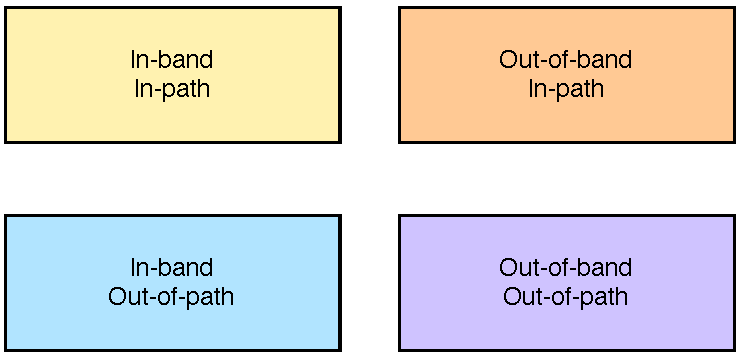
\includegraphics[width=0.9\columnwidth]{chap2-fw-outline}
\caption{Classification of Congestion cues~\cite{Singh:PhDFw}}
\label{fig:4:fw}
\end{figure}

A congestion control algorithm needs to pick one or more measurement points,
picking multiple adds to the feedback overhead and then choose a method to
signal it to the sending endpoint. It can choose to report it in-band by
encapsulating the cues either by piggybacking them on endpoint's own media
packets as RTP header extensions (this adds to the header overhead of a media
packet) or as RTCP extension blocks (see section~\ref{fw.freq} for details on
feedback frequency). Or the congestion control algorithm can choose to signal
the cues out-of-band, i.e., re-use the signaling path (e.g., SIP, XMPP) or
setup an alternate signaling path (e.g., HTTP or websockets). Following are
the examples for each category in the classification:

\textbf{\texttt{a) In-path, In-band}}: TFRC using information in RTCP RR, TFRC
using additional loss reported by ECN markings, Temporary Maximum Media Stream
Bit Rate Request (TMMBR), Receiver Estimated Max Bit rate (REMB).

\textbf{\texttt{b) In-path, Out-of-band}}: RTSP implements a SPEED parameter
to vary the transmission rate, announcing bandwidth in the SDP.

\textbf{\texttt{c) Out-of-path, In-band}}: Multipath RTP (congestion on one
path causes a change in the fractional distribution of traffic on each path.)

\textbf{\texttt{d) Out-of-path, Out-of-band}}: bandwidth/congestion
notifications from congestion maps, bandwidth lookup service, super-peers and
overlays.

% monitoring: long-term, short-term

% Additionally if the cue reliably
% describes the onset of congestion (\emph{knee}) or the collapse
% (\emph{cliff}).

% \begin{figure}[!h]
% 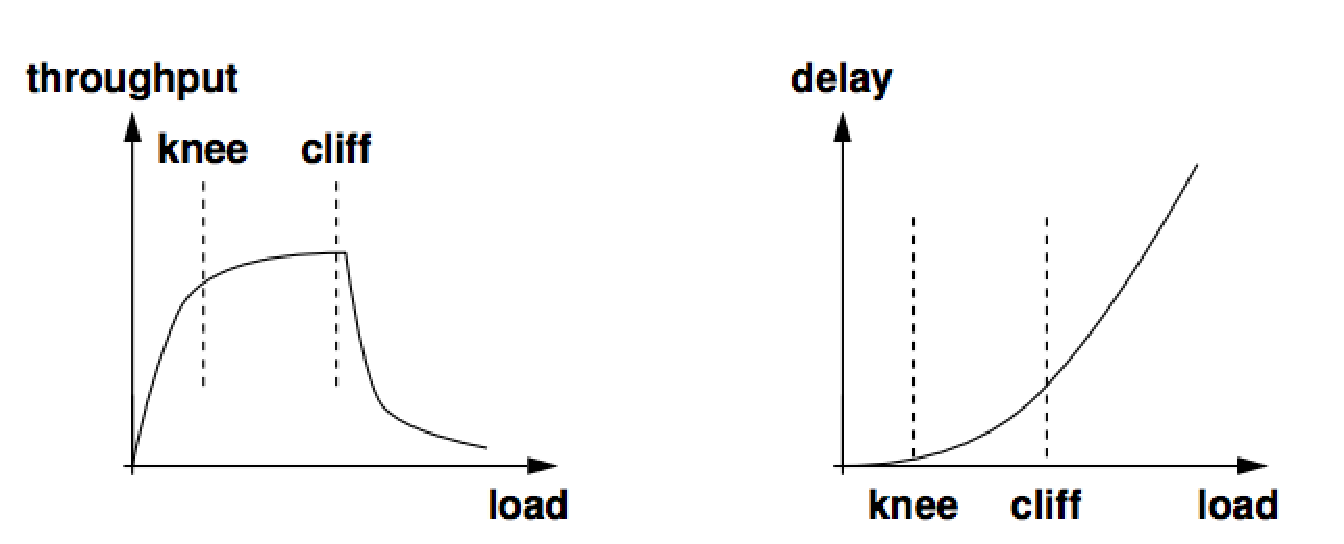
\includegraphics[width=\columnwidth]{chap4-knee-cliff}
% \caption{Shows the variation throughput and delay with increasing network load}
% \label{fig:4:knee}
% \end{figure}

\section{Congestion Control Evaluation}
\label{fw.cc.eval}

We need to define a set of requirements in order to design a congestion
control algorithm for multimedia. As a second step these requirements are used
as a checklist to evaluate the suitability of the proposed algorithms. Real-
time interactive communication differs greatly from \emph{elastic} traffic
because the sender generates media packets in real-time and expects it to be
delivered in 100s of milliseconds and the receiver consumes the media packets
almost immediately, hence late arriving packets are useless. Additionally,
real-time communication systems are able to tolerate some amount of packet
loss and adapt the media rate over a fairly large range.
\cite{draft.rmcat.req} lists a set of requirements for RTP-based interactive
multimedia sessions, these requirements form the basis of the guidelines
described in~\cite{draft.rmcat.evaluate}.  We define a catalogue of
\emph{traffic flows} traversing through a \emph{network topology} with varying
\emph{link characteristics} and diverse \emph{queuing} strategies. By picking
one feature from each category in the category, we construct scenarios to
evaluate the performance of the congestion control. The evaluation scenarios
are built using the following components: network topology, link and router
characteristics.

\subsection{Network flows}

\begin{enumerate}
\setlength{\itemsep}{5pt}

\item \textbf{\texttt{Single media flow on an end-to-end path}}: this scenario
describes the best case, wherein the network puts each flow identified by its
5-tuple (protocol, source and destination IP address, source and destination
port numbers) on its own queue, thereby the flow using the proposed congestion
control algorithm does not encounter any cross-traffic.

\item \textbf{\texttt{Single media flow competing with the similar flows}}: in
this scenario, the flow using the proposed congestion control algorithm
competes with flows using the same congestion control algorithm (i.e., all
flows are interactive multimedia).


\item \textbf{\texttt{Single media flow competing with TCP}}: in this
scenario, the flow using the proposed congestion control algorithm competes
with TCP flows. These maybe \emph{short} TCP flows representing common
web-traffic patterns or \emph{long} TCP flows depicting bulk transfers (e.g.,
large file downloads).

\end{enumerate}

% In Section~\ref{rg.title}, we describe the network traffic scenarios to
% evaluate the proposed congestion control algorithms, namely, when the flows
% are a) alone, b) competing with self-similar flows, and c) competing with TCP
% flows (short-, long-lived) on a bottleneck link.




\subsection{Link characteristics}

The link characteristics can be broken down into the following categories:
throughput, latency, loss. Throughput of a link typically only varies in
wireless networks, for example in 3G, LTE, WLAN, etc. In Wireless LAN (WLAN)
networks it may also vary depending on the density of nodes using the network.

Next, latency of a link is the propagation and serialization delay. Queuing
delay is based on the queue-size of the router and hence, a router
characteristic. Latencies between nodes typically varies between a few
milliseconds up to 100s of milliseconds. Commonly used values are: LAN (very
low delay, $<1$ms), Low delay ($<40$ms), trans-continental ($>100$ms), or
Satellite links ($>500$ms).

Packet losses are modeled using the Gilbert-Elliott
Model~\cite{gilbert1960capacity, elliott1963estimates} or by packet
traces~\cite{ellis:2011:dataset, 3gppSim}.


\subsection{Router characteristics}

 % Queue-size and Queue type.

Apart from managing packet routing, a router also manages congestion; when a
packet arrives at a higher rate than it can process the packet, it queues the
packet. The routers then use \emph{priority queuing}, \emph{fair queuing}, or
\emph{weighted fair queuing (WFQ)}~\cite{rfc4594} to decide which traffic
class to transmit or drop packets from during congestion. When congestion
occurs within the same traffic class the router discards packets using
\emph{tail drop}, \emph{Random Early Detection (RED)}~\cite{Floyd:RED} or
\emph{Weighted Random Early Detection (WRED)}.

We describe the queue sizes as a function of time, i.e., it is the depth of
the queue or the amount of time the packet will remain in the queue before it
is discarded. However, in practice the queue size is measured in number of
packets. We convert the queue depth (measured in time) to queue length (number
of packets, MTU is typically 1500 bytes) using:

\begin{equation*}
  \mathrm{QueueSize}_\mathrm{packets} = 
    \frac{\mathrm{QueueSize}_\mathrm{sec} \times
    \mathrm{Throughput}_\mathrm{bps}}{\mathrm{MTU} \times \mathrm{8}}
\end{equation*}

For example, a router with a throughput of 1Mbps and a 1s queue depth would be
capable of handling 83 packets (queue length). For example, the 100ms queue
depth may represent a short queue, while the 10s queue depth represents a
buffer-bloated queue.

\subsection{Network topology}

We should run different types of network topologies to evaluate the
performance of congestion control. Chiefly, the location of the bottleneck
link helps in gauging the performance of the congestion control. Depending on
the amount of cross-traffic the bottleneck link will move from one node to
another in the network. Also the bottleneck in each direction may be different
due to the asymmetry of access links. Additionally, the varying capacity of
the access link (e.g., in wireless environments) may be the bottleneck.

Figure~\ref{fig:4:topology} shows an example of the evaluation setup. This
topology is commonly called the \emph{dumb-bell} topology. Another common
topology is \emph{parking lot}, which uses multiple bottleneck instead of a
single bottleneck; however, both use common concepts. 


To define a scenario, we need to choose the following: pick the cross-traffic,
define the characteristics of the cross traffic (self-similar, short- or
long-lived TCP). Define the characteristics of the edge routers (Router X and
Y) and introduce impairments to the bottleneck link. Lastly, measure and
analyze the performance of the multimedia system. 

% We typically use dummynet~\cite{Carbone:2010p3502} or NetEm~\cite{netem} or
% packet traces~\cite{s4.eval.bitrate} to emulate the variation in link
% capacity, latency, intermediate router queue length, and packet losses.

\begin{figure}[!h]
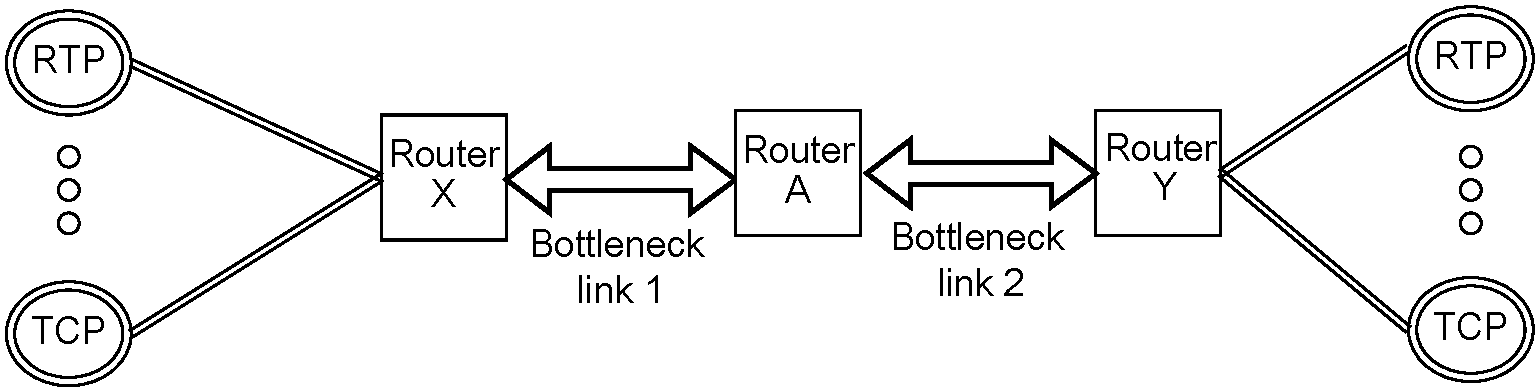
\includegraphics[width=\columnwidth]{chap4_fig_sim_topology}
\caption{Typical network topology for evaluating congestion control;
		 it consists of traffic flows (evaluating flow and cross 
		 traffic), links and routers.}
\label{fig:4:topology}
\end{figure}



\section{Circuit Breakers for Unicast RTP Sessions}

Due to media flow's (chiefly due to video) high data rate, if congestion
control is not implemented by multimedia applications, they can cause severe
congestion in the network, especially in low capacity networks. This can
disrupt multimedia's quality of experience and other applications on the
network.

We are developing a circuit breaker algorithm that can work with unmodified
RTP applications, and determine when these non-adaptive multimedia
applications are causing excessive network congestion and cease their
transmission.  We envision that the congestion control algorithms for
multimedia standardized in the IETF will need to work inside the envelope of
this circuit breaker algorithm~\cite{draft.rmcat.evaluate}. Hence, the circuit
breakers cannot be too aggressive in terminating media flows because it
should allow sufficient time for the congestion control algorithm  to monitor
and respond to congestion cues.

The circuit breaker algorithm in the short term will serve as a policer,
during which time the congestion control algorithm is developed. Developing
standard congestion control algorithms for unicast RTP-based interactive
multimedia applications is expected to be a multi-year process at the IETF.
Consequently, the development of the circuit breaker is on a tight schedule,
to be ready for inclusion in the initial roll out of the WebRTC (Web-based
Real-time Communication) framework~\cite{jennings:2013:webrtc} in web
browsers.

\subsection{Circuit Breaker Design}

The RTP circuit breaker algorithm relies on the basic feedback mechanisms
defined in the RTP Control Protocol (RTCP)~\cite{rfc3550}. That is, it solely
uses the information available in the RTCP Sender Report (SR) and Receiver
Report (RR) packets to detect if the flow is overusing the capacity or causing
congestion.

Common congestion indicators are: 1) the network \emph{round trip time} (RTT)
calculated  using timing information in RTCP SR and RR packets, 2)
\emph{jitter} estimated by the receiver over the last reporting interval, and
3) fractional packet loss and cumulative \emph{loss} reported by the receiver
during the last RTCP interval. These indicators  unfortunately only provide a
limited insight into the behavior of the network and cannot be used as strong
signals for a circuit breaker.

Variation in RTT is used as a congestion indicator in delay-based congestion
control  algorithms. Additionally, some algorithms use RTT estimates to
configure connection timeouts. In RTP/RTCP, the RTT is estimated infrequently
because the feedback intervals are rather long making it difficult to detect
the cause in  variation of delay. Likewise, variation in jitter can indicate a
transient network congestion but do not  provide a strong signals to implement
a circuit breaker. On the other hand, loss is a strong indicator of congestion
in networks where  packet losses predominantly occur due to queue overflows
and less accurate indicator where packet loss can occur due to bit-error
corruption (e.g., wireless  and mobile links). Therefore, we base the circuit
breaker conditions on packet losses. They are:

\begin{enumerate}
\setlength{\itemsep}{5pt}

\item \textbf{\texttt{Media Timeout}}: An endpoint is sending media data but
the receiver reports a non-increasing \emph{Highest Sequence Number} (HSN) for
two consecutive RTCP intervals the flow is terminated.

\item \textbf{\texttt{RTCP Timeout}}: An endpoint is sending media data but
receives no RTCP RR for three consecutive RTCP intervals the flow is
terminated.

\item \textbf{\texttt{Congestion}}: An endpoint is sending media data and
receives RTCP RRs indicating fractional packet loss, it calculates the TCP
friendly rate and compares it to the sending rate. If the sending rate exceeds
the TCP friendly rate  by a factor of 10 for two consecutive RTCP intervals
the flow is terminated.

\end{enumerate}

Full details of the RTP circuit breaker algorithm is discussed
in~\cite{draft.rtp.cb}, it is a work in progress and covers various deployment
cases such as multiple media sources, impact of shorter than standard
reporting interval, deployment of Explicit Congestion Notification (ECN), etc.

In \citepub{c:cb}, we apply these circuit breaker conditions to non-adaptive
RTP media flows. Such flows typically do not implement congestion control at
this time, and are likely to cause congestion if deployed on the Internet. We
carried out a series of experiments based on real-world traces and on a
test-bed emulating real-world conditions. Our results show that the proposed
RTP circuit breaker performs well, triggering in cases of bursty loss and in
sessions that are congesting the links, and does not trigger in low-loss and
non-bursty scenarios. 

We simulated RTP circuit breaker performance on $3833$ generated RTCP traces
corresponding to the measurements collected in \emph{dataset-A} and
\emph{dataset-B} of~\cite{ellis:2011:dataset}. Of these, $1626$ traces have no
packet loss, and hence cannot trigger the RTP circuit breaker. The remaining
traces each include at least one lost packet. We categorize the remaining
traces into two categories: those that have non-bursty packet loss; and those
that exhibit bursty loss using the definition of bursty loss
from~\cite{rfc3611} (Figure~\ref{fig:bursty} shows representative samples of
the non-bursty and bursty packet loss patterns). The data comprises $1344$
traces with bursty loss, $863$ traces with non-bursty loss.

\begin{figure}
  \centerline{
    \subfloat[Non-bursty]{
      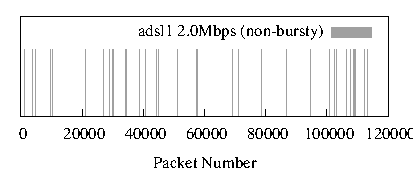
\includegraphics[width=0.5\columnwidth]
      {chap4_graph_cb_20090707-1515-barcode}
    }
    \subfloat[Bursty]{
      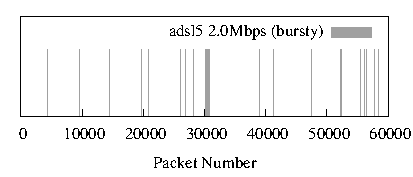
\includegraphics[width=0.5\columnwidth]
      {chap4_graph_20091011-2012-barcode}
    }
  }
  \caption{Sample bursty and non-bursty packet loss traces.}
  \label{fig:bursty}
\end{figure}

\begin{table}
  \begin{center}
    \begin{tabular}{rcc}
    \toprule
    Loss Pattern       & Triggered & Did not trigger \\
    \midrule
             Loss free &   0.0\% & 100.0\% \\
       Non-bursty loss &   0.0\% & 100.0\% \\
          Bursty loss  &  11.9\% &  88.1\% \\
    \bottomrule
    \end{tabular}
    \caption{Sessions triggering circuit breaker by loss pattern}
    \label{tab:cb_bursty}
  \end{center}
\end{table}

Table~\ref{tab:cb_bursty} shows the fraction of sessions that triggered the
RTP circuit breaker for each of the categories of packet loss. The RTP circuit
breaker did not trigger for sessions without loss; it also did not trigger for
any of the sessions with non-bursty packet loss. However, we observe that the
RTP circuit breaker is triggered more often in sessions that contain bursty
packet loss.


The circuit breaker conditions trigger mainly due to loss,
Figure~\ref{fig:short-rtcp} shows the percentage of sessions triggering the
circuit breaker increases with the increase in loss rate. The figure also
shows the impact of the RTCP reporting interval, i.e., by reducing the RTCP
interval from 5s to 2.5s, fewer sessions are terminated. The endpoints become
robust to loss of feedback packets by sending feedback often and we observe
a longer time to trigger the circuit breaker ($t_{CB}$).

\begin{figure}
  \centerline{
    {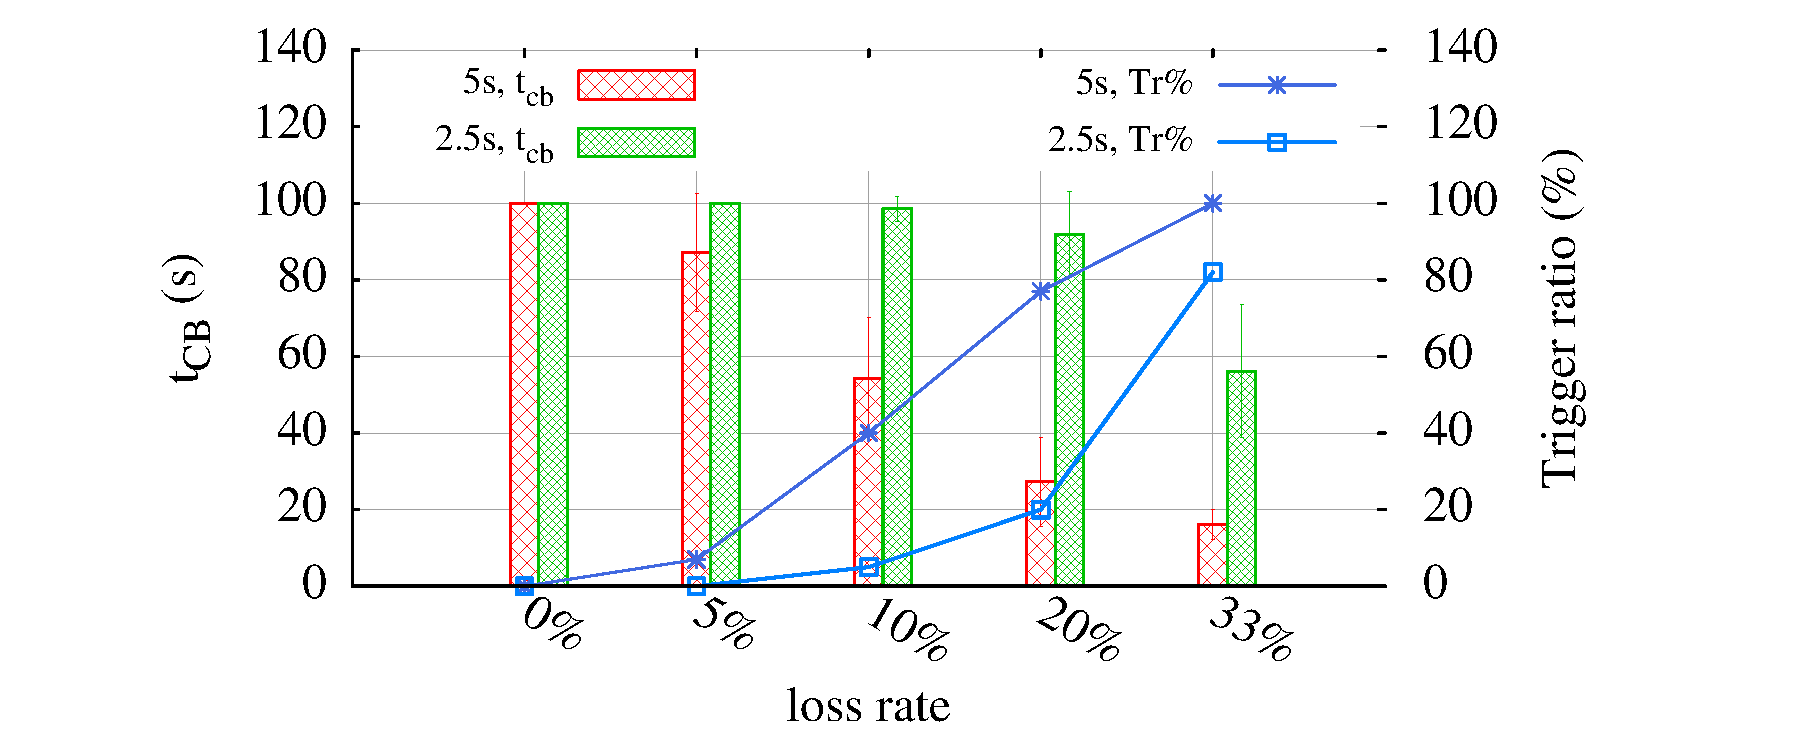
\includegraphics[width=\columnwidth]{chap4_graph_cb_cmp_trr_2s}}
  }
  \caption{Impact of using a shorter RTCP interval on the circuit breaker. 
    Each scenario is run 50 times and the error bars represent the $95\%$ 
    confidence level.}
  \label{fig:short-rtcp}
\end{figure}
